\documentclass[conference]{IEEEtran}
\IEEEoverridecommandlockouts
% The preceding line is only needed to identify funding in the first footnote. If that is unneeded, please comment it out.
\usepackage{cite}
\usepackage{amsmath,amssymb,amsfonts}
\usepackage{algorithmic,algorithm}
\usepackage{graphicx}
\graphicspath{ {./images/} }
\usepackage{textcomp}
\usepackage{xcolor}
\usepackage{lettrine}
\usepackage{lipsum,booktabs}

\def\BibTeX{{\rm B\kern-.05em{\sc i\kern-.025em b}\kern-.08em
    T\kern-.1667em\lower.7ex\hbox{E}\kern-.125emX}}
\begin{document}

\title{SpotifyClassifier: Music Genre Classification with Big Data\\
}

\author{\IEEEauthorblockN{1\textsuperscript{st} Alex Thornton}
\IEEEauthorblockA{\textit{Dept. of Electrical Engineering} \\
\textit{Columbia University}\\
New York, USA \\
apt2141@columbia.edu}
\and
\IEEEauthorblockN{2\textsuperscript{nd} Elmira Aliyeva}
\IEEEauthorblockA{\textit{Dept. of Computer Science} \\
\textit{Columbia University}\\
New York, USA \\
ae2970@columbia.edu}
\and
\IEEEauthorblockN{3\textsuperscript{rd} Tanvi Pande}
\IEEEauthorblockA{\textit{Dept. of Electrical Engineering} \\
\textit{Columbia University}\\
New York, USA \\
tp2673@columbia.edu}
}

\maketitle
\thispagestyle{plain}
\pagestyle{plain}
\begin{abstract}
Music genre classification is a complex task, which can even be difficult for humans. Using a Spotify Developer account to interface with their API, we have created our own dataset and a music genre classifier capable of identifying song genres for individual tracks. We leveraged Spotify's pre-processed track metadata, allowing for genre classification with only a song name as an input, rather than an audio mp3 file. Additionally, we performed novel research into subgenre connectivity by comparing overlap between cross classified songs.
\end{abstract}

\begin{IEEEkeywords}
Music, Classification, Hierarchal Learning, Machine Learning, Big Data Analytics, Supervised Learning
\end{IEEEkeywords}

\section{Introduction}
\lettrine{E}{ach} December 1\textsuperscript{st}, social media explodes with a "Spotify Wrapped" summary of users' preferences over the past year. Individual users can post to Instagram or Tik Tok about their top artists, tracks, genres, as well as more abstract concepts like music aura. Currently, Spotify's API can only provide genre labels for artists, not specific tracks. Our team has combined the power of the Spotify Developer API with big data tools such as Google Cloud Computing, Apache Spark, and machine learning techniques to solve this problem. 

Considering the widespread interest and proliferation of "Spotify Wrapped" posts in 2021, there is a clear business value for being able to predict the genre tastes of individual users, particularly their favorite songs. However, Spotify providing genre labels for only artists does not provide enough granularity. Consider the example of a listener of Taylor Swift enjoying \emph{Trouble (Taylor's Version)} on her 2021 re-release of her popular album \emph{Red (Taylor's Version)}. What genre would this song be classified as? Spotify might be able to point you to an array of genres that Taylor Swift has performed over her career, but this is a very broad list! Entire albums across her discography vary greatly tonally, lyrically, and musically. Figure \ref{fig:TSwiftie} illustrates the vast difference between \emph{Red (Taylor's Version) (2021)} and \emph{Reputation (2017)}.

\begin{figure}[htbp]
\centerline{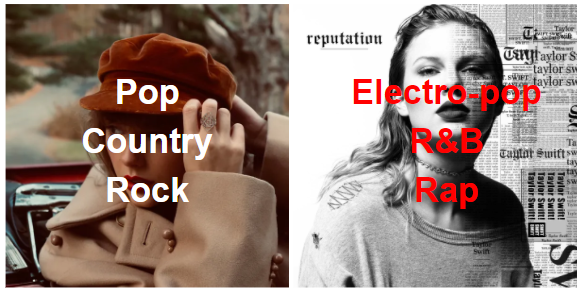
\includegraphics[width=9cm]{images/TSwiftie.png}}
\caption{Red (Taylor's Version) vs. Reputation}
\label{fig:TSwiftie}
\end{figure}

We suspect that on their application backend, Spotify has genre classifications for individual tracks. However, they are likely not providing all their information publicly, and are treating some subset of their data as trade secret. This suspicion is further supported by "Spotify Wrapped" including genres that are not supported for their Developer API. Spofity only supports 126 genres with their Developer API, but have been known to classify music into over 1,300 micro-genres like "grave-wave" and "metropolis" \cite{b1}. To uncover some of the magic of Spotify's classification algorithms, we built our own dataset of labelled tracks using their 'recommendation' feature, and used machine learning to reverse engineer a classification algorithm of our own. 

\section{Related Work}

Starting in 2002,  G. Tzanetakis and P. Cook attempted to use k-nearest neighbors models to perform genre classification on 3 broad genre sets, with an accuracy of around 61\% \cite{b2}. A more recent academic project out of Stanford's CS229 Machine Learning class was able to increase this amount to 80\% for 10 genres, using a CNN trained on the Short Time Fourier Transform (STFT) of song mp3 files from the publicly available GTZAN dataset of 1000 songs \cite{b3}. These examples are able to achieve decent accuracy, as human performance on classification across this range of high level genres is usually around 70\% \cite{b4}.

A more interesting application also comes out of Stanford's CS229 Machine Learning class was able to classify across 4 distinct genres (Christian, Country, Jazz, Metal) by processing the album art, lyrics, and a small audio sample of songs, which they procured using the Spotify Developer API. Processed features were then fed through a recurrent neural network (RNN), Naive Bayes, and other models to achieve over 90\% accuracy \cite{b5}. While this is excellent accuracy, the genre selection they used isn't very useful or broad.

Suppose that a user wants to classify the genre of a specific track, but doesn't have access to an mp3 file. The previous examples would be useful if a large enough dataset of mp3 files was labelled, and the user would always have a copy of the music they want to classify. However, the very existence of Spotify as a streaming service indicates a growing movement to separate users from the actual data itself, as opposed to audio marketplace and storage solutions of the early 2000's like iTunes. A much more likely scenario would be a use case where a user knows the name of a track they want to classify, but don't actually own or possess a copy of the music. A clunky implementation for this use case might scrape YouTube and illegally convert the audio to a mp3, then run the raw data through one of the previously mentioned genre classification models. While this might suffice for a proof of concept, we prefer to do things by the book.

Our method embraces big data and the plethora of publicly available metadata through the Spotify Developer API, and can fetch metadata and classify based on the name of a track alone. While genre classification itself isn't a novel application of machine learning, this use case is. Using the Spotify API, our team built our own dataset that leverages over 30,000 individual songs, from 73 distinct genres, and ambitiously has set out to classify genres using this broader, big data approach.

\section{Data}
\subsection{Data Collection}
One of the unique aspects of Spotify's Developer API is its 'recommendation' feature, which can be used to find music that matches a number of criteria, including genres. As of December 2021, Spotify supports a total of 126 genres for recommendation. While Spotify doesn't provide the genre labels for individual tracks, they are able to recommend up to 100 specific tracks for a given seed genre. By requesting recommendations for each supported genre in a loop, and saving off non-repeat tracks until a sufficient number were collected, we were able to construct a labelled dataset of tracks, their Spotify ID, and a corresponding genre label. 

\begin{figure}[htbp]
\centerline{\includegraphics[width=9cm]{images/pitch.png}}
\caption{Audio filter for pitch vectorization \cite{b6}}
\label{fig:pitch}
\end{figure}

After tracks were collected and organized with genre labels, we went back to Spotify to collect metadata to serve as features for our model. Available audio features include scores for abstract concepts like 'danceability' to more concrete, quantitative values like tempo and loudness. Features were saved to a json file for each track, and stored in a Google Cloud Storage project. 

\begin{figure}[htbp]
\centerline{\includegraphics[width=9cm]{images/timbre.png}}
\caption{Timbre basis function \cite{b6}}
\label{fig:timbre}
\end{figure}

In addition to pre-processed audio features, we also leveraged Spotify's 'Audio-Analysis' and 'Track-Info' calls. Track info is straightforward, allowing us to collect the year of release and relative popularity of tracks, which actually serve as excellent discriminators. A lot more people are listening to Ed Sheeran in 2021 than Mozart, and classic rock music is much more likely to correlate to music written in the 1980s. Audio analysis calls provide in depth analysis of tracks, with 1x12 vectors for each musically distinct 'segment' of a song for pitch and timbre. As songs can have vastly different numbers of unique segments depending on song length, we averaged pitch and timbre to get consistent 1x12 vectors as features. Figures \ref{fig:pitch} and \ref{fig:timbre} show a visual representation of these vectors.

\subsection{Genre Hierarchy}

With a class of genres so large, we clustered 73 of the 126 genres as subgenres under larger 'super-genres'. For example, grunge, emo, and indie could all be subgenres of the 'alternative' super-genre. Initially, we expected to classify based on both super-genre and subgenre, with performance on the former being much better. However, as discussed in the Analysis section, subgenre classification was much more difficult than anticipated. 

\begin{figure}[htbp]
\centerline{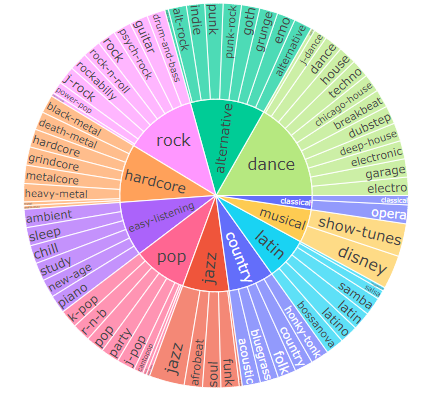
\includegraphics[width=8cm]{images/GenreHierarchy.PNG}}
\caption{Super-genre hierarchy of subgenres}
\label{fig:GenreHierarchy}
\end{figure}

\begin{figure*}
  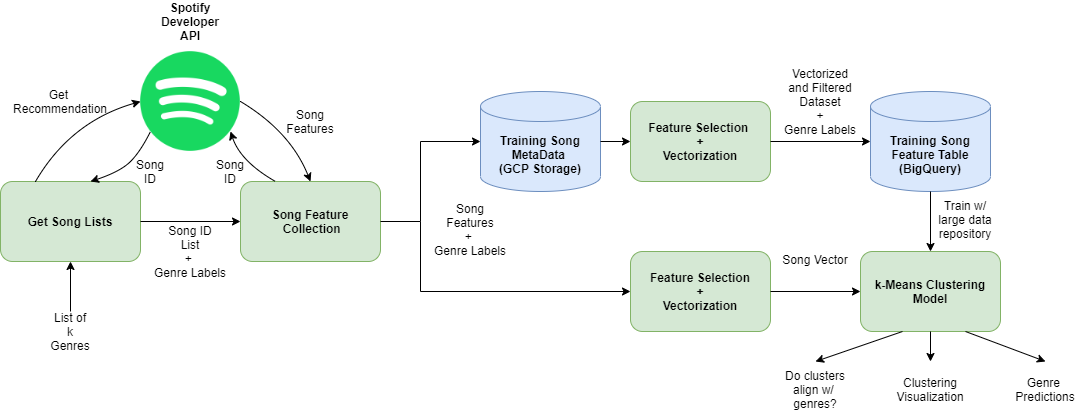
\includegraphics[width=\textwidth]{images/SystemArchitecture.png}
  \caption{System architecture}
  \label{fig:architecture}
\end{figure*}

Approximately 500 songs were collected for each subgenre, creating as balanced a dataset as possible. We realized through trial and error that while many subgenres were able to produce almost 1000 unique tracks after a few hundred API calls (and throwing away repeats each time), some subgenres only had the same 100 tracks for every API call. We ended up tossing out subgenre seeds with only 100 tracks to offer, whittling the 126 supported genres to 73 that had enough tracks and could be categorized nicely into super-genres. We also found that 500 tracks was a good target for track count per subgenre.

An important distinction is that some subgenres could fall under multiple super-genres, like punk-rock being split across alternative and rock. For simplification, we mapped each subgenre to only one super-genre. This simplification would prove problematic later, but served as a solid first pass. The super-genre hierarchy used is shown in Figure \ref{fig:GenreHierarchy}, displayed as a sunburst diagram with subgenres branching radially from their respective super-genre. Additionally, the scale of the diagram is accurate for relative track count between genres within our dataset. The number of samples per subgenre, and number of subgenres per super-genre were carefully selected to create as balanced a dataset as possible.

\section{System Overview}
The system architecture is defined in Figure \ref{fig:architecture}, with scripts in green, cloud storage in blue, and front end in purple. Data collection, as described in previous sections, interacts directly with the Spotify Developer API. Track lists are compiled from recommendations for supported seed genres, and features are collected for each of those tracks. From here, we leveraged Colab / Jupyter notebooks, Google Cloud nodes, and Apache Spark to vectorize and store the features as json files for each song, in directories by subgenre. 

Data from cloud storage was converted to tables in BigQuery, so that we could easily prep and load training, and validation data. We went with an 80:20 split across every subgenre for training / validation. A number of machine learning models were tested against our training data to find the best model for our application, and the \emph{Methods} section describes the results for individual models. This trained model is saved and stored on our Github repository for easy loading into the application.

\begin{figure}[htbp]
\centerline{\includegraphics[width=8cm]{images/Application.png}}
\caption{Mock-up of front end application}
\label{fig:application}
\end{figure}

A stretch goal for our team was to have the end user only interact with the simple purple block, with a clean design and intuitive design. The user enters the track they want to classify into a search bar, and on the back end, we determine the closest match for that track with the Spotify 'Search' call. The features are collected and vectorized similarly as with the training data, and passed through the pre-trained machine learning model for classification. We ended up running out of time for the live demo getting the front end connected to the back end, but do have a mock-up of what an application might look like, as shown in Figure \ref{fig:application}.

\section{Methods}
\subsection{Machine Learning Models}
When we first set out to do this project, we had planned on doing an unsupervised learning application for classification. We would find 100,000 tracks, unlabelled genres, and do k-means clustering on the features of tracks to find hidden patterns. However, after digging deeper into the Spotify Developer API, we determined that it actually would be possible to create our own genre labels with the aformentioned process, so we pivoted our approach to a supervised learning application. 

\begin{table}[h]
  \centering
  \caption{Machine Learning Model Performance}
  \label{tab2}
  \begin{tabular}{@{}p{3cm}l@{}}
    \toprule
    \multicolumn{1}{}{}Model & Our architecture\\
    \midrule
    Random Forest Classifier                        & .4765 \\
    Decision Tree Classifier                        & .4156 \\
    Logistic Regression                             & .5518 \\
    LinearSVC                                       & .4796 \\
    GBT Classifier                                  & .6223 \\
    \bottomrule
  \end{tabular}
\end{table}


After prepping the features by track for our new dataset, we used it to train a number of machine learning models. The results of our findings for various models is seen in Table I. Gradient Boosted Trees performed the best of the ML models over the 11 super-genres tested, with accuracy around 62\%. Further metrics for the GBT model can be seen in Table II. We estimate that the delta between this performance and the benchmark of 70\% for humans to be because of the lossy data. Since we aren't using a real mp3 file and are only relying on pre-processed metadata, some information will naturally get lost in translation. We do some deeper digging into improving this performance in the analysis section, re-thinking the super-genre hierarchy model we adopted, and considering the reliability of the subgenre labels provided by Spotify. 

\begin{table}[h]
  \centering
  \caption{Gradient-Boosted Trees Performance}
  \label{tab2}
  \begin{tabular}{@{}p{3cm}l@{}}
    \toprule
    \multicolumn{1}{}{}Metric & Score\\
    \midrule
    F1-Score                        & .6217 \\
    Precision                       & .6238 \\
    Recall                          & .6223 \\
    Accuracy                        & .6223 \\
    \bottomrule
  \end{tabular}
\end{table}

\subsection{Final Model Performance}
\begin{figure}[htbp]
\centerline{\includegraphics[width=8cm]{images/TrainingConfusion.PNG}}
\caption{Training confusion matrix}
\label{fig:TrainingConfusion}
\end{figure}

As anticipated, the super-genre hierarchy simplification to organize our dataset isn't perfect. In particular, our model struggled with differentiating between alternative and rock super-genres. This makes a lot of sense, because alternative could have even been a subgenre of rock, and they sound very similar. The training and test confusion matrices in Figures \ref{fig:TrainingConfusion} and \ref{fig:TestConfusion} confirm that result, as well as the surprise that jazz was difficult to categorize, our model mis-classified everything but hardcore and classical for jazz tracks. In the context of music history, rock, pop, r&b, and latin music draws a lot of inspiration from jazz music, so this isn't entirely surprising.

\begin{figure}[htbp]
\centerline{\includegraphics[width=8cm]{images/TestConfusion.PNG}}
\caption{Test confusion matrix}
\label{fig:TestConfusion}
\end{figure}

\section{Analysis}
As previously mentioned, using the super-genre hierarchy described in Figure \ref{fig:GenreHierarchy} has its limitations. Clearly, there are some super-genres that are closely related and difficult to distinguish. But an important observation is that the super-genre labels were created by us, Spotify only provided the subgenre labels. Perhaps we oversimplified a complex relationship between the subgenres by grouping them under one definitive super-genre. Consider the example of a song classified as punk-rock. Would this song be classified under 'alternative' or 'rock' with our model? Either label is sufficient, but only one is 'correct' under our model, which is an oversimplification for sure. We predicted that a better model for grouping the subgenres would look something like Figure \ref{fig:NaiveOverlap}, with clusters of super-genres connected together by borderline subgenres.

\begin{figure}[htbp]
\centerline{\includegraphics[width=9cm]{images/SupergenreGraphSquare.PNG}}
\caption{Our naive subgenre overlap model}
\label{fig:NaiveOverlap}
\end{figure}

Re-framing the problem as a graph problem allows both for data analysis as well as new solutions. For example, the approach we took was to re-group subgenres or throw away 'unreliable' subgenres from the dataset. Another approach might look at determining some notion of edge weights between subgenre nodes in the graph, and updating our loss model for classification to be weighted vectors by subgenre connectivity instead of 'all or nothing' one-hot encoding. We determined a procedure (Algorithm 2) for the latter, which we describe in the Future Works section, but leave its implementation as an exercise for the reader.

\subsection{Search for Subgenre Inter-Connectivity}
Out of the 73 genre seeds we derived our dataset from, some provide more information than others. For instance, tracks with the 'opera' subgenre label were hardly ever categorized as anything other than the 'classical' super-genre, so that label provides high information. A traditional way to think about the information provided by each subgenre would be to frame the supergenre as an unbiased estimator of a subgenre random variable as a function of the track features, and to determine the Fisher Information of each label. This isn't practical, because the subgenres are discrete and disjoint. Instead, we determined a new metric, \emph{Inter-Connectivity-Rank}, to compare how frequently specific subgenres overlap with other subgenres. Subgenres with a high \emph{Inter-Connectivity-Rank} are the most difficult to categorize into a single super-genre, and are therefore less reliable as labels. We expected that subgenres which had lower classification accuracy would show up at the top of this ranking.

\subsection{What is this, a Crossover Episode?}
To find how to define this new metric, and establish a concrete algorithm to compute it, we started digging into the data. Elmira first noticed that there was a significantly non-trivial number of tracks that were recommended by Spotify for more than one subgenre, some as many as nine different subgenres! Modern alternative bands tended to be the worst offenders, with Blink-182, Mumford \& Sons, and MGMT all producing tracks that Spotify recommended for at least six different seed genres, as shown in Figure \ref{fig:Crossover}.

\begin{figure}[htbp]
\centerline{\includegraphics[width=9cm]{images/Crossover.png}}
\caption{Album art for tracks associated with multiple subgenres from Blink-182, Mumford \& Sons, and MGMT}
\label{fig:Crossover}
\end{figure}

\subsection{The Inter-Connectivity-Rank Algorithm}
After we collected a list of tracks that appeared in multiple subgenre lists, we set out to formulate the 
\emph{Inter-Connectivity-Rank} for our dataset. For every track that was listed multiple times, we formed
a 'cluster' of the subgenres that were associated with that track. From there, we determined how many 
times that subgenre appeared in a cluster, and ranked them. Additionally, we calculated an edge matrix,
with subgenres as the vertices, as a boolean if subgenre $i$ ever appeared in a cluster with subgenre $j$.
The procedure for performing these operations is described in detail in Algorithm 1.

\begin{algorithm} 
\textit{S := data structure of subgenres, with track features organized by subgenre}
\newline
\textit{I := sorted dictionary of interconnectivity rank by subgenre}
\newline
\textit{E := boolean edge matrix for all subgenres}
\newline
\textt{ (I,E) = Inter-Connectivity-Rank(s)}
\newline
\begin{algorithmic}[H]
\caption{Inter-Connectivity-Rank}
\STATE I $\gets$ dictionary of zero for all subgenres
\STATE T $\gets$ empty list
\FOR{all $s \in S$}
\FOR{all track-id in s}
\STATE T.append (track-id, subgenre) 
\ENDFOR
\ENDFOR
\STATE T $\gets$ (elements of T with $>$ 1 appearance of track-id)
\STATE subgenre-clusters $\gets$ empty hash table
\FOR{ all $t \in T$}
\STATE subgenre-clusters[t[track-id]].append(t[subgenre])
\ENDFOR
\STATE E $\gets$ array of \emph{False} for all subgenres, dimension S x S
\FOR{cluster in subgenre-clusters}
\FOR{all s in cluster}
\STATE I[s] += 1
\ENDFOR
\FOR{all pairs i,j of subgenres in cluster}
\IF {E[i,j] == \emph{False}} 
\STATE E[i,j] = \emph{True}
\ENDIF
\ENDFOR
\ENDFOR
\STATE I[s] = reverse-sort-by-value(I[s])
\RETURN (E, I)
\end{algorithmic}
\end{algorithm}

After computing the \emph{Inter-Connectivity-Rank} for each subgenre, we compiled a list of the top 10 most inter-connected subgenres, as shown in Figure \ref{fig:Ranking}. As anticipated, 'alternative', 'punk-rock', and 'rock-n-roll' all make an appearance. Surprisingly, 'chill', 'study', and 'sleep' round out the top 10. Interestingly, these three were all part of our 'easy-listening' super-genre. We determined that the easy-listening category was far too broad, and tossed it from the dataset, resulting in an accuracy improvement of a small percentage. 'Study' and 'Chill' aren't really genres, but verbs the user performs while listening to music of many genres. We probably wouldn't have come to this conclusion without doing this analysis, so we're convinced the \emph{Inter-Connectivity-Rank} is a useful metric for this type of analysis. 

\begin{figure}[htbp]
\centerline{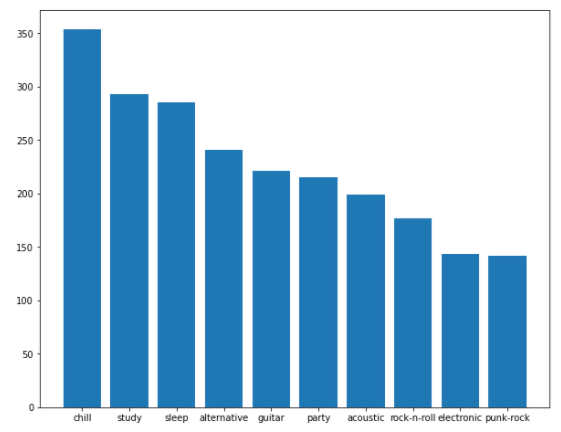
\includegraphics[width=9cm]{images/TopOffenders.png}}
\caption{Top-10 inter-connected subgenres}
\label{fig:Ranking}
\end{figure}

Other unsurprising offenders appearing in the top 10 are 'guitar', 'party', and 'acoustic'. These are definitely genres and not verbs like with the easy-listening subgenres, but they are incredibly vague. Guitar for example could easily be rock, alternative, hardcore, country, and pop. Surprising or 
otherwise, we decided to toss these highly overlapping subgenres from the dataset. We included an updated 
sunburst diagram in Figure \ref{fig:UpdatedHierarchy} to display our dataset after tossing the top 10 
ranking subgenres.

\begin{figure}[htbp]
\centerline{\includegraphics[width=8cm]{images/UpdatedGenreHierarchy.PNG}}
\caption{Updated super-genre hierarchy of subgenres}
\label{fig:UpdatedHierarchy}
\end{figure}

\subsection{Inter-Connectivity Visualized}

\begin{figure*}
  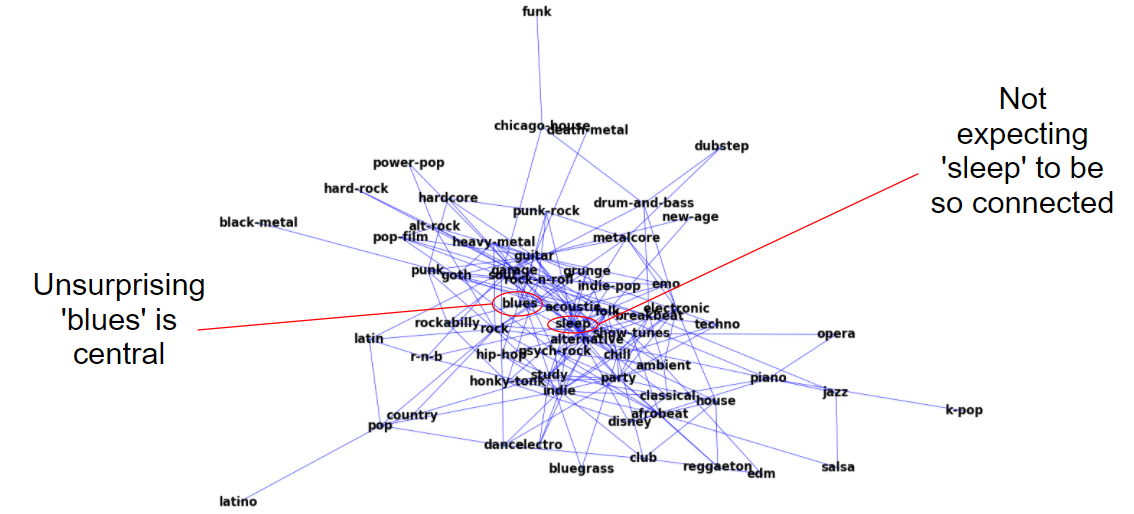
\includegraphics[width=\textwidth]{images/Analysis.PNG}
  \caption{True subgenre inter-connectivity structure}
  \label{fig:Analysis}
\end{figure*}

In addition to a ranking of subgenres, the \emph{Inter-Connectivity-Rank} algorithm also returned
the edge matrix defining edges between subgenres of the cross-labelled songs in our dataset. Using the
networkx Python package, we were able to visualize the output of the algorithm as a graph, as seen
in Figure \ref{fig:Analysis}. This is another way to see the \emph{Inter-Connectivity-Rank} of the 
subgenres, and reveals the same information we saw before. It's unsurprising that subgenres like 
'blues' and 'alternative' appear toward the center, with many edges. But the top offenders like
'sleep' and 'chill' are also near the exact center as well. 

The subgenres with the lowest \emph{Inter-Connectivity-Rank} are easier to see. 'Black-metal', 'latino', and 'k-pop' are clear outliers in the graph, with only one connection each. Some other subgenres from the hardcore supergenre also appeared completely unconnected to the rest of this graph entirely. This aligns
with the results we saw in the Methods section, where the hardcore super-genre had very high accuracy.
The connection between our graph here and the results seen by our model confirms that the subgenres with
the lowest \emph{Inter-Connectivity-Rank} were the most distinguishing for classification, and therefore provided the most information as a label. 

\section{But Wait - There's More}
This project provided an excellent application as well as some interesting and novel analysis, but there still is quite a lot left to explore in this field that would make this project even better. Clearly, getting the front end shown in Figure \ref{fig:application} was a stretch goal for us, so that would be priority one in future work beyond this paper. But the possibilities go much further than getting Tanvi's Javascript app to cooperate with our model. 

\subsection{Improved Inter-Connectivity-Rank Algorithm}
At the start of the Analysis section, we teased a second, improved \emph{Inter-Connectivity-Rank} algorithm that would improve model performance and serve as a more interesting visual. After thinking about our Algorithm 1, which produced the \emph{Inter-Connectivity-Ranking} and Figure \ref{fig:Analysis}, we determined that there might be some information lost in translation given the way we were processing the repeated tracks. Consider the edge case that 'salsa' is cross listed with 'dance' very frequently, but never cross listed with any other subgenres. Given Algorithm 1, it could happen that 'salsa' and 'dance' could emerge at the top of the ranking, despite only ever being linked with each other! 

In Algorithm 1 for \emph{Inter-Connectivity-Ranking}, we computed the ranking based on the number of cross-listed track subgenre clusters each subgenre appears in. But as pointed out in the edge case, this is biased for subgenres that are frequently coupled with a small group of subgenres. Even if 'emo' and 'goth' are often cross listed with each other, they share the parent super-genre 'alternative', so their high correlation doesn't impact the information we can derive. A better algorithm would be able to differentiate subgenres based not on the number of collisions, or cross-correlations with any subgenre, but the number of unique collisions. This can be computed as the number of unique outgoing edges for each subgenre from the $E$ matrix derived in Algorithm 1.

Another way to improve Algorithm 1 would be to better define the edges in the produced graph structure. Previously, we defined the edge matrix as boolean, so if a collision between two subgenres appeared only once in all the cross-listed tracks, it would count the same as a collision between two subgenres appearing one thousand times. It might be useful to track the number occurrence's each edge gets counted, so an improved algorithm would track that as well. The layout for Algorithm 2 is provided below.

\begin{algorithm} 
\textit{S := data structure of subgenres, with track features organized by subgenre}
\newline
\textit{I := sorted dictionary of interconnectivity rank by subgenre}
\newline
\textit{E := boolean edge matrix for all subgenres}
\newline
\textt{ (I,E) = Improved-Inter-Connectivity-Rank(s)}
\newline
\begin{algorithmic}[H]
\caption{Improved-Inter-Connectivity-Rank}
\STATE I $\gets$ dictionary of zero for all subgenres
\STATE T $\gets$ empty list
\FOR{all $s \in S$}
\FOR{all track-id in s}
\STATE T.append (track-id, subgenre) 
\ENDFOR
\ENDFOR
\STATE T $\gets$ (elements of T with $>$ 1 appearance of track-id)
\STATE subgenre-clusters $\gets$ empty hash table
\FOR{ all $t \in T$}
\STATE subgenre-clusters[t[track-id]].append(t[subgenre])
\ENDFOR
\STATE E $\gets$ array of $0$ for all subgenres, dimension S x S
\FOR{cluster in subgenre-clusters}
\FOR{all pairs i,j of subgenres in cluster}
\STATE E[i,j] += 1
\ENDFOR
\ENDFOR
\FOR{all i in E[i,j]}
\FOR{all j in E[i,j]}
\IF{ E[i,j] $\geq$ 1}
\STATE{I[s[i]] += 1}
\ENDIF
\ENDFOR
\ENDFOR
\STATE I = reverse-sort-by-value(I)
\RETURN (E, I)
\end{algorithmic}
\end{algorithm}
\raggedbottom
\subsection{Improved Label Encoding \& Loss Function}
Not only will Algorithm 2 provide better data visualization, but we expect it to significantly improve model performance. Right now, labels for super-genres are one-hot encoded, so for a 5 super-genre subset of our data given by ['alternative', 'rock', 'hip-hop', 'jazz', 'country'], a valid representation for a track labelled 'rock' could be given by:

\begin{figure}[ht]
\centering
$Y=
\begin{bmatrix}
0\\
1\\
0\\
0\\
0\\
\end{bmatrix}
$
\end{figure}

Consider how the edge matrix $E$ could help augment this. Perhaps there would be a count of 250 between 'alternative' and 'rock', and 50 between 'hip-hop' and 'rock', with the max element of $E$ being 500. We could normalize the edge counts relative to the maximum edge, and multiply by a factor $\alpha $ so that we could account for subgenre overlap, while not diluting the original label. 

For example, let $\alpha=\frac{1}{2}$,

\begin{figure}[ht]
\centering
$\hat{Y}=
\begin{bmatrix}
0+\alpha*\frac{250}{500}\\
1\\
0+\alpha*\frac{50}{500}\\
0\\
0\\
\end{bmatrix}
=
\begin{bmatrix}
\frac{1}{4}\\
1\\
\frac{1}{20}\\
0\\
0\\
\end{bmatrix}
\rightarrow
\hat{Y_{normalized}} = 
\begin{bmatrix}
.192\\
.769\\
.039\\
0\\
0\\
\end{bmatrix}
$
\end{figure}

By using this as a new subgenre label, and using a mean square error loss function for training and accuracy metrics, we can account for subgenre overlap. Not only would this improve our accuracy in training and test, but would also allow us to make better genre predictions. Instead of our model delivering one genre prediction, it would instead output a normalized vector of genre ratios. This way, a track split across two or more super-genres could be represented correctly, rather than forced under one label.

\subsection{Expanded Features}
As mentioned in \emph{Related Work}, a music genre classifier from Stanford's CS229 class (that was also integrated into the Spotify Developer API) was able to use album art, lyrics, and a sample of audio as features for individual tracks \cite{b5}. From our experience, the availability of the audio snippets is spotty from genre to genre, often being unavailable for less popular genres. However, album art and lyrics are almost always available. Using a CNN to process features from album art, and a RNN language model for the lyrics could add two additional highly discriminatory features to each track, and improve model performance.

\pagebreak
\section{Conclusion}
Every year, Big Data continues to make waves in all areas of society, and music is no exception. Just 10 years ago, streaming music was a radical idea, with a large market share of listeners relying on personal libraries of digital copies of their music. Spotify has likely permanently changed the music industry forever, ushering in the era of streaming, listener profiling, and AI informed music recommendation. 

We expect that AI will continue to transform the user experience for music streaming, and "Spotify Wrapped" is just the beginning in visually and audibly exciting data analytics to optimize the user experience. Our application likely only re-invented the wheel of some of the magic under the hood of the Spotify ML algorithms for music classification, but our novel approach to subgenre inter-connectivity provides a fresh take to improve any dataset with ambiguous and dependent labels, with implications far beyond the subset of music classification problems.

\begin{figure}[htbp]
\centerline{
\includegraphics[width=8cm]{images/logo.png}}
\caption{SpotifyClassifier Logo}
\label{fig:logo}
\end{figure}


\pagebreak
\section*{Thank You!}
Thank you to Professor Ching-Yung Lin, and TA's Cong Han, Yvonne Lee, Guoshiwen Han, Yiwen Fang for your support throughout EECS E6983, and your ideas for this project. We appreciate you.

Thank you also to AJ Johnson of Lockheed Martin, and Samuel Stone of SRC inc. for their feedback in preparing and improving this project.


\pagebreak
\begin{thebibliography}{00}
\bibitem{b1} N. Patch, Meet the man classifying every genre of music on Spotify, thestar.com. 2016.
\bibitem{b2} G. Tzanetakis and P. Cook. Musical genre classification of audio signals. IEEE Transactions on Speech and Audio Processing, 10(5):293–302, July 2002.
\bibitem{b3} D. Huang, A. Serafini, E. Pugh, \emph{Music Genre Classification}, 2018, Accessed on December 21, 2021. [Online]. Available: \url{http://cs229.stanford.edu/proj2018/report/21.pdf}
\bibitem{b4} Mingwen Dong. Convolutional neural network achieves human-level accuracy in music genre classification. CoRR, abs/1802.09697, 2018.
\bibitem{b5} T. Dammann, K. Haugh, \emph{Genre Classification of Spotify Songs using Lyrics, Audio Previews, and Album Artwork}, 2017, Stanford University
\bibitem{b6} Spotify Developer API Documentation - Track Audio Analysis, Accessed on December 21, 2021. [Online]. Available: \url{ https://developer.spotify.com/documentation/web-api/reference/#/operations/get-audio-analysis}

\end{thebibliography}

\section*{Further Acknowledgements}
Album artwork referenced for Taylor Swift, Blink-182, Mumford \& Sons, and MGMT.
\pagebreak
\section*{One More Thing}
To Taylor Swift,
\newline
\newline
Listening to your music while writing this paper at 2 A.M. 
is what got me through. 
\newline
\newline
Thank you.
\newline
\newline
-Alex

\end{document}

